\documentclass[a4paper, 12pt]{article}

\usepackage[top=2cm, bottom=2cm, left=2.5cm, right=2.5cm]{geometry}
\usepackage[utf8]{inputenc}
\usepackage{amsmath, amsfonts, amssymb}
\usepackage{graphicx} % inserir figuras - \includegraphics[scale=•]{•}
\usepackage{float} % ignorar regras de tipografia e inserir figura aonde queremos.
\usepackage[brazil]{babel} % Trocar Figure para Figura.
\usepackage{indentfirst}
\pagestyle{empty}


\begin{document}
\begin{figure}[htb]
	
\includegraphics[scale=0.9]{UnB_CiC_Logo.jpg}
\end{figure}
\noindent\rule{\textwidth}{0.4pt}
\begin{center}
	\textbf{{\Large Introdução à Ciência da Computação - 113913}} \newline \newline
	\textbf{{\large Lista de Exercícios 4} \\
	\vspace{9pt}
	{\large Funções Frutíferas}} \\
	\noindent\rule{\textwidth}{0.4pt}
	\newline
\end{center}

\textbf{{\large Observações:}}
\begin{itemize}
	\item As listas de exercícios serão corrigidas por um \textbf{corretor automático}, portanto é necessário que as entradas e saídas do seu programa estejam conforme o padrão especificado em cada questão (exemplo de entrada e saída). Por exemplo, não use mensagens escritas durante o desenvolvimento do seu código como ``Informe a primeira entrada''. Estas mensagens não são tratadas pelo corretor, portanto a correção irá resultar em resposta errada, mesmo que seu código esteja correto.
	\item As questões estão em \textbf{ordem de dificuldade}. Cada lista possui 7 exercícios, sendo 1 questão fácil, 3 ou 4 médias e 2 ou 3 difíceis.
	\item Assim como as listas, as provas devem ser feitas na versão Python 3 ou superior.
	\item Leia com atenção e faça \textbf{exatamente} o que está sendo pedido.
\end{itemize}
\newpage % Questão A 
\begin{center}
\textbf{{\Large Questão A - Função de Comparação}}
\end{center}
\vspace{5pt}
Escreva uma \textbf{função} \textbf{\textit{compare}} que dado dois números \textbf{\textit{x}} e \textbf{\textit{y}}, retorne 1 se x for maior que y, 0 se for igual a y, e -1 se x for menor que y. Usando o retorno da função, imprima na tela: ``x e maior que y'' se o retorno for 1, ``x e igual a y'' se o retorno for 0, e ``x e menor que y'', caso contrário.
\newline \newline
\textbf{{\large Entrada}} \newline
Duas linhas de entrada correspondentes aos inteiros \textbf{\textit{x}} e \textbf{\textit{y}}.
\newline \newline
\textbf{{\large Saída}} \newline
Será impresso na tela a mensagem ``x e maior que y'' se o retorno da função for 1, ``x e igual a y'' se o retorno da função for 0, e ``x e menor que y'', caso contrário.
\newline
\begin{table}[H]
	\centering
	\begin{tabular}{|l|l|}
	\hline
	\textbf{Exemplo de Entrada} & \textbf{Exemplo de Saída} \\ \hline
	\begin{tabular}{l}
	4 \\
	5
	\end{tabular} & x e menor que y \\ \hline
	
	\begin{tabular}{l}
	3 \\
	3
	\end{tabular} & x e igual a y \\ \hline
	
	\begin{tabular}{l}
	-1 \\
	-2
	\end{tabular} & x e maior que y \\ \hline
	
	\end{tabular}
	\caption{Questão A}
	\label{tabela1}
\end{table}

\newpage % Questão B
\begin{center}
\textbf{{\Large Questão B - Função para Entrada de Dados}}
\end{center}
\vspace{5pt}
\textbf{Usando uma função}, faça um programa que leia 10 números inteiros e imprima
na tela o maior deles. No caso de valores iguais, imprima qualquer um dos
maiores. Caso o maior número seja múltiplo do primeiro número \textbf{\textit{n}} lido, imprima \textbf{\textit{n}} na tela.
\newline \newline
\textbf{{\large Entrada}} \newline
Dez números inteiros, considere que o primeiro número lido nunca será 0.
\newline \newline
\textbf{{\large Saída}} \newline
O maior número \textbf{\textit{maior}} e o primeiro número \textbf{\textit{n}} lido, caso
$m = a \cdot n, a\in \mathbb{Z}$.
\newline
\begin{table}[H]
	\centering
	\begin{tabular}{|l|l|}
	\hline
	\textbf{Exemplo de Entrada} & \textbf{Exemplo de Saída} \\ \hline
	\begin{tabular}{l}
	3 \\
	1 \\
	2 \\
	3 \\
	4 \\
	5 \\
	6 \\
	7 \\
	8 \\
	9
	\end{tabular} & 
	\begin{tabular}{l}
	9 \\
	3
	\end{tabular} \\ \hline
	
	\begin{tabular}{l}
	-1 \\
	-5 \\
	-4 \\
	10 \\
	8 \\
	0 \\
	4 \\
	3 \\
	2 \\
	1
	\end{tabular} & 
	\begin{tabular}{l}
	10 \\
	-1
	\end{tabular} \\ \hline
	
	\begin{tabular}{l}
	-2 \\
	-4 \\
	-8 \\
	-16 \\
	-32 \\
	-64 \\
	-128 \\
	-256 \\
	-512 \\
	-2
	\end{tabular} & 
	\begin{tabular}{l}
	-2 \\
	-2
	\end{tabular} \\ \hline
	\end{tabular}
	\caption{Questão B}
	\label{tabela2}
\end{table}

\newpage % Questão C
\begin{center}
\textbf{{\Large Questão C - Pares do Intervalo}}
\end{center}
\vspace{5pt}
\textbf{Usando recursividade}, faça um programa que dado um inteiro \textbf{\textit{n}} positivo lido do
teclado, retorne todos os números pares maiores ou iguais a dois, que são
menores ou iguais a \textbf{\textit{n}}.
\newline \newline
\textbf{{\large Entrada}} \newline
Um único inteiro $\textrm{\textbf{n}} \geq \textrm{\textbf{0}}$.
\newline \newline
\textbf{{\large Saída}} \newline
Todos os números pares, maiores ou iguais a zero, que são menores ou iguais a
\textbf{\textit{n}}, um por linha.
\newline
\begin{table}[H]
	\centering
	\begin{tabular}{|l|l|}
	\hline
	\textbf{Exemplo de Entrada} & \textbf{Exemplo de Saída} \\ \hline
	10 & \begin{tabular}{l}
	10 \\
	8 \\
	6 \\
	4 \\
	2
	\end{tabular} \\ \hline
	
	15 & \begin{tabular}{l}
	14 \\
	12 \\
	10 \\
	8 \\
	6 \\
	4 \\
	2
	\end{tabular} \\ \hline
	
	4 & \begin{tabular}{l}
	4 \\
	2 \\
	\end{tabular} \\ \hline
	\end{tabular}
	\caption{Questão C}
	\label{tabela3}
\end{table}

\newpage % Questão D
\begin{center}
\textbf{{\Large Questão D - Soma de Sequência Par}}
\end{center}
\vspace{5pt}
Usando \textbf{funções recursivas}, faça um programa que dado um inteiro \textbf{\textit{n}} lido do
teclado, retorne e imprima na tela a soma de todos os números pares de 0 até
\textbf{\textit{n - 2}}, incluindo \textbf{\textit{n - 2}}, se for o caso. Caso \textbf{\textit{n}} seja menor que 0, imprima na tela ``-1''.
\newline \newline
\textbf{{\large Entrada}} \newline 
Um único inteiro \textbf{\textit{n}}.
\newline \newline
\textbf{{\large Saída}} \newline
Será impresso na tela a soma de todos os pares de 0 até \textbf{\textit{n - 2}}. Caso \textbf{\textit{n}} seja menor que 0 o programa deverá imprimir -1 na tela.
\newline
\begin{table}[H]
	\centering
	\begin{tabular}{|l|l|}
	\hline
	\textbf{Exemplo de Entrada} & \textbf{Exemplo de Saída} \\ \hline
	15 & 42 \\ \hline
	20 & 90 \\ \hline
	-1 & -1 \\ \hline
	\end{tabular}
	\caption{Questão D}
	\label{tabela4}
\end{table}

\newpage % Questão E
\begin{center}
\textbf{{\Large Questão E - Quadrado de Pares}}
\end{center}
\vspace{5pt}
Usando funções faça um programa que leia um valor \textbf{n indefinidas vezes}. O
programa deve encerrar quando o valor de \textbf{\textit{n}} for zero. Para cada \textbf{\textit{n}} lido apresente o quadrado de cada um dos valores pares (conforme formato especificado
abaixo) de 1 até \textbf{\textit{n}}, inclusive \textbf{\textit{n}}, se for o caso.
\newline \newline
\textbf{{\large Entrada}} \newline
Inteiro $\textrm{\textbf{n}} \geq \textrm{\textbf{0}}$.
\newline \newline
\textbf{{\large Saída}} \newline
Será impresso na tela o quadrado de todos os números pares de 1 até \textbf{\textit{n}} que são menores ou iguais a \textbf{\textit{n}}, conforme exemplo abaixo.
\newline
\begin{table}[H]
	\centering
	\begin{tabular}{|l|l|}
	\hline
	\textbf{Exemplo de Entrada} & \textbf{Exemplo de Saída} \\ \hline
	\begin{tabular}{l}
	7 \\
	0
	\end{tabular} & \begin{tabular}{l}
	6\^{}2 = 36 \\
	4\^{}2 = 16 \\
	2\^{}2 = 4
	\end{tabular} \\ \hline
	
	\begin{tabular}{l}
	1 \\
	2 \\
	0
	\end{tabular} & \begin{tabular}{l}
	2\^{}2 = 4
	\end{tabular} \\ \hline
	
	\begin{tabular}{l}
	10 \\
	5 \\
	3 \\
	0
	\end{tabular} & \begin{tabular}{l}
	10\^{}2 = 100 \\
	8\^{}2 = 64 \\
	6\^{}2 = 36 \\
	4\^{}2 = 16 \\
	2\^{}2 = 4 \\
	4\^{}2 = 16 \\
	2\^{}2 = 4 \\
	2\^{}2 = 4
	\end{tabular} \\ \hline	
	
	\end{tabular}
	\caption{Questão E}
	\label{tabela5}
\end{table}

\newpage % Questão F
\begin{center}
\textbf{{\Large Questão F - Mínimo Múltiplo Comum}}
\end{center}
\vspace{5pt}
O mínimo múltiplo comum (mmc) de dois inteiros \textbf{\textit{a}} e \textbf{\textit{b}} é o menor inteiro positivo que é múltiplo simultaneamente de \textbf{\textit{a}} e de \textbf{\textit{b}}. Se não existir tal inteiro positivo, por exemplo, se \textbf{\textit{a = 0}} ou \textbf{\textit{b = 0}}, então \textbf{\textit{mmc(a,b)}} é zero por definição. O mínimo múltiplo comum é útil em operações de soma e subtração de frações vulgares, onde é preciso um denominador comum entre as frações operadas. \textbf{Usando recursividade} faça um programa que leia dois números separados por espaço indefinidas vezes e calcule o seu mmc. O programa deve encerrar quando a entrada conter um número negativo.
\newline \newline
\textbf{{\large Entrada}} \newline
Cada linha de entrada conterá dois inteiros \textbf{\textit{a}} e \textbf{\textit{b}}.
\newline \newline
\textbf{{\large Saída}} \newline
O mínimo múltiplo comum de \textbf{\textit{a}} e \textbf{\textit{b}}.
\newline
\begin{table}[H]
	\centering
	\begin{tabular}{|l|l|}
	\hline
	\textbf{Exemplo de Entrada} & \textbf{Exemplo de Saída} \\ \hline
	\begin{tabular}{l}
	8 12 \\
	20 24 \\
	3 9 \\
	-1 0
	\end{tabular} & \begin{tabular}{l}
	24 \\
	120 \\
	9
	\end{tabular} \\ \hline
	
	\begin{tabular}{l}
	4 5 \\
	2 7 \\
	13 3 \\
	-5 -5
	\end{tabular} & \begin{tabular}{l}
	20 \\
	14 \\
	39
	\end{tabular} \\ \hline
	
	\begin{tabular}{l}
	4 4 \\
	0 4 \\
	7 133 \\
	4 90 \\
	0 -10
	\end{tabular} & \begin{tabular}{l}
	4 \\
	0 \\
	133 \\
	180
	\end{tabular} \\ \hline	
	\end{tabular}
	\caption{Questão F}
	\label{tabela6}
\end{table}

\newpage % Questão G
\begin{center}
\textbf{{\Large Questão G - Definição Recursiva de Strings}}
\end{center}
\vspace{5pt}
Seja uma \textbf{string s} definida da seguinte forma: $$s::= nil \mid n:s' $$onde \textbf{\textit{nil}} representa a string vazia, e \textbf{\textit{n:s'}} denota a string com primeiro elemento \textbf{\textit{n}} e cauda \textbf{\textit{s'}} (sendo s' também uma string). \newline 
O comprimento de uma string é definido recursivamente por:
$$length(s) =
		\begin{cases}
			0;\, \textrm{se}\ s = nil \\
			1 + length(s');\, \textrm{se}\ s = a:s' \\
		\end{cases}
$$
A concatenação de strings também pode ser definida por uma função recursiva:
$$concat(s1,s2) =
		\begin{cases}
			s2;\, \textrm{se}\ s1 = nil \\
			a:(concat(s1',s2));\, \textrm{se}\ s1 = a:s1' \\
		\end{cases}
$$
O reverso de strings é definido por:
$$rev(s) =
		\begin{cases}
			s;\, \textrm{se}\ s = nil \\
			concat(rev(s'), (n:nil));\, \textrm{se}\ s = n:s' \\
		\end{cases}
$$
Uma lista é prefixo da outra se:
$$prefix(s1,s2) =
		\begin{cases}
			True;\, \textrm{se}\ s1 = nil\, \textrm{e}\  s2 \neq nil\\
			prefix(s1', s2');\, \textrm{se}\ s1 = a:s1'\, \textrm{e}\ s2 = a:s2' \\
			False;\ \textrm{caso contrário}
		\end{cases}
$$
Considerando o código dado abaixo e usando as definições recursivas acima, \textbf{complete} o programa abaixo.
\begin{figure}[H]
	\centering
	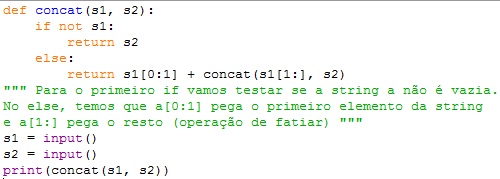
\includegraphics[scale=0.75]{strings.png}
\end{figure}
Dado duas strings \textbf{\textit{s1}} e \textbf{\textit{s2}}, o trecho de código acima escreve na tela parte do que é especificado em \textbf{Saída}. \newline \newline
\textbf{{\large Entrada}} \newline
A entrada consistirá apenas de duas strings \textbf{\textit{s1}} e \textbf{\textit{s2}}. \textbf{Não terá como entrada duas strings iguais.}
\newline \newline
\textbf{{\large Saída}} \newline
Escreva na tela s1 concatenada com s2, o reverso de s1 e se s1 é prefixo de s2. \textbf{No primeiro exemplo s1 é a string vazia (nil).}
\newline
\begin{table}[H]
	\centering
	\begin{tabular}{|l|l|}
	\hline
	\textbf{Exemplo de Entrada} & \textbf{Exemplo de Saída} \\ \hline
	\begin{tabular}{l}
	 \\
	b
	\end{tabular} & \begin{tabular}{l}
	b \\
	 \\
	True
	\end{tabular} \\ \hline
		
	\begin{tabular}{l}
	aaa \\
	bbb
	\end{tabular} & \begin{tabular}{l}
	aaabbb \\
	aaa \\
	False
	\end{tabular} \\ \hline

	\begin{tabular}{l}
	cd \\
	cdd
	\end{tabular} & \begin{tabular}{l}
	cdcdd \\
	dc \\
	True
	\end{tabular} \\ \hline
	
	\end{tabular}
	\caption{Questão G}
	\label{tabela7}
\end{table}
\end{document}